\begin{savequote}[72mm]

I think the brain is essentially a computer and consciousness is like
a computer program. It will cease to run when the computer is turned
off. Theoretically, it could be re-created on a neural network, but
that would be very difficult, as it would require all one's memories.

\qauthor{Stephen Hawking}
\end{savequote}

\chapter{Introducción}
\label{cha:Introducción}

\graphicspath{{1_introduction/images/}}

La motivación de escribir un libro sobre redes neuronales nace a
partir de que es un tema que ido desarrollando como parte de mi
formación como Científico de la Computación, así como ser uno de los
modelos de \textsl{\gls{aprendizajemaquina}} que más han sido
investigados en los últimos años y que más fascinación me han dado.\\

Este libro no pretende ser más que una guía para comprender como
implementar redes neuronales artificiales usando un lenguaje funcional
(\gls{clojure}), tratando de reproducir resultados como el perceptrón
simple \cite{rosenblatt1958perceptron} o los mapas autoorganizados de
Kohonen \cite{kohonen1982som, Kohonen2001}. Esto se pretende llevar a
partir del estudio matemático de las distintas redes y enfocarlos en
el desarrollo de aplicaciones de software.

\section{¿Qué es una red neuronal artificial?}

Las redes neuronales artificiales son un enfoque computacional basado
en un conjunto de unidades de procesamiento que están interconectadas
entre sí de forma similar en que las conexiones biológicas del cerebro
están conectadas y se usan para resolver distintos tipos de problemas
relacionados con el aprendizaje, clasificación o clusterización de
información.\\

Generalmente cada neurona artificial (en adelante sólo
\textit{neurona}), está conectada con otras y sus conexiones pueden
ser activar o inhibir otras neuronas. Cada neurona determinar estas
activaciones o inhibiciones a partir de una función matemática que
está definida en término de sus entradas (conexiones), las cuáles al
evaluarse en la función y llegar a cierto umbral disparan la
activación o inhibición de la neurona, siendo esta activación o
inhibición la salida de la función con valores discretos o continuos.\\

A la forma en que se encuentran conectadas las neuronas entre sí, lo
vamos a denominar \textsl{\gls{arquitectura}}. Esta ``Arquitectura''
es el modo en que las neuronas pueden compartir información. Las
formas habituales en que se distribuyen las neuronas es a través de
capas de neuronas, las cuales se agrupan en en unidades
estructurales. Distinguiremos tres tipos de capas, de entrada, de
salida y oculta.\\

\begin{itemize}
\item \textbf{Capa de entrada}: Corresponde con la capa sensorial,
  encargada de recibir datos o señales del entorno.
\item \textbf{Capa de salida}: Es el conjunto de neuronas que proveen
  los resultados del procesamiento de los datos o señales de la red.
\item \textbf{Capa oculta}: Es una capa que no está conectada con el
  entorno, generalmente sirve para proveer representaciones internas
  del entorno.
\end{itemize}

Procederemos ahora a dar una definición formal de lo que es una red
neuronal:

\theoremstyle{definition}
\begin{definition}
  Una red neuronal es un grafo dirigido con las siguientes
  características:
  \begin{enumerate}
  \item A cada vértice \textsl{i} se asocia a una variable de estado
    $x_i$
  \item A cada conexión $(i,j)$ de los vértice $i$ y $j$ se le asocia un
    peso $w_{ij} \in \mathbb{R}$
  \item A cada vértice $i$ se le asocia un umbral $\theta_i$
  \item Para cada vértice $i$ se define una función $f_i(x_j, w_{ij},
    \theta_i)$ que va a depender de las conexión, del umbral y de los
    estados de los $j$ a el conectados. Esta función define el nuevo
    estado del vértice.
  \end{enumerate}
\end{definition}

Habitualmente, las redes neuronales se clasifican en dos tipos de
operación o aprendizaje, siendo estos el aprendizaje supervisado y el
aprendizaje no supervisado, los cuáles hablaremos con mayor detalle en
las siguientes secciones.

\textbf{Incluir imágenes para ilustrar el contenido anterior}

\section{Aprendizaje de la red neuronal}

En el contexto de las redes neuronales se entiende como
\textbf{aprendizaje} al proceso de adaptación de la red neuronal en el
que adapta sus parámetros internos de la red a través de estímulos
externos. Comúnmente el aprendizaje consiste en determinar un conjunto
de pesos sinápticos que permita a la red realizar correctamente el
procesamiento pretendido.\\

El modo convencional de aprendizaje es definiendo una regla de
aprendizaje $\Delta w_{ij}$ definida en términos de la conexión
$w_{ij}$ que representa la conexión del peso de la neurona
presináptica de la neurona $j$ con la postsináptica $i$ en la
iteración $t$, quedando de la siguiente forma:

\begin{equation}
  \Delta w_{ij}(t+1) = w_{ij}(t) + \Delta w_{ij}(t)
\end{equation}

El proceso de aprendizaje es iterativo, actualizándose los pesos hasta
que la red neuronal alcanza el rendimiento de procesamiento deseado.\\

Los modelos comunes de aprendizaje son el aprendizaje supervisado y el
aprendizaje no supervisado. Existen otros como el aprendizaje híbrido
o el aprendizaje reforzado que no van a ser tratados aquí.

\subsection{Aprendizaje supervisado}

De manera informal se puede hablar del aprendizaje supervisado como la
presentación a la red de patrones, junto a la salida deseada u
objetivo, de tal modo que la red ajuste sus pesos hasta que la salida
sea tan similar como la que fue presentada previamente. De este modo
la red es capaz de estimar relaciones entrada/salida sin proponer una
cierta forma funcional de inicio.

\subsection{Aprendizaje no supervisado}

El aprendizaje no supervisado se puede describir de forma general como
la estimación de la función de densidad de probabilidad $p(x)$ que va
a describir la distribución de patrones x correspondientes al espacio
de entrada $\mathbb{R}^n$ a partir de ejemplos. \\

En este tipo de aprendizaje, se presenta a la red una gran cantidad de
patrones sin que nosotros le indiquemos cual es la salida deseada. La
red a través de la regla de aprendizaje va intentar extraer rasgos del conjunto de entrada.

\section{Breve historia de las redes neuronales}

Durante mucho tiempo ha existido un encanto en tratar de modelar los
distintos procesos cognitivos del cerebro a través de mecanismos de
hardware. Ejemplos de estas primeras construcciones las podemos
encontrar durante la Segunda Guerra Mundial con la construcción de la
máquina Enigma [\textbf{Agregar referencia}] utilizada para la
codificación de mensajes entre las tropas alemanas.\\

En 1943, el neurofisiólogo Warren McCulloch y el matemático Walter
Pitts escriben un artículo sobre el posible funcionamiento de las
neuronas cerebrales modelándola como una red neuronal simple usando
circuitos electricos \cite{mcculloch1943logical}.\\

En 1950, Alan Turing propone una pregunta que dice: «\texttt{¿Pueden
 las máquinas pensar?}» \cite{turing1950computing} influyendo en la
visión de la inteligencia artificial como una imitación del
comportamiento humano, pero esto no tuvo el exito esperado, si no
siendo más dominante la visión de que la inteligencia artificial debe
ser más como un comportamiento racional.\\

\begin{wrapfigure}{l}{0.25\textwidth}
    \centering
    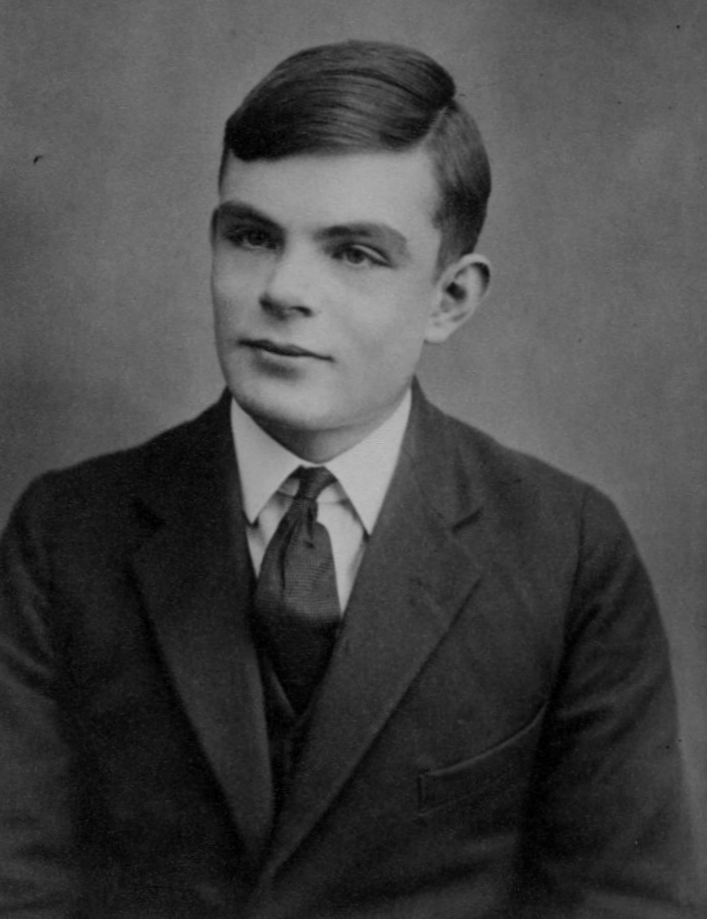
\includegraphics[width=0.25\textwidth]{Alan_Turing}
    \caption{Alan Turing a los 16 años}
    \label{fig:turing}
\end{wrapfigure}

En 1958, Frank Rossenblatt propone el \textbf{Perceptrón Simple}
como un dispositivo electrónico construido para mantener los
principios biológicos de una neurona y la habilidad para aprender. En
1962 publicó un libro llamado «\texttt{Principles of
 neurodynamics. Perceptrons and the theory of brain mechanisms}» en
que extendió y desarrolló sus investigaciones sobre el perceptrón,
utilizando este libro como apoyo para sus cursos \cite{rosenblatt1958perceptron}.\\

En 1962, Bernard Widrow y Marcian Hoff desarrollan modelos llamados
\textbf{ADALINE} y \textbf{MADALINE}, donde ADALINE fue desarrollada
para reconocer patrones binarios. Mientras que MADALINE fue la primer
red neuronal aplicada a un problema de la vida real, utilizando un
filtro adaptativo para eliminar el echo en las lineas telefónicas
\cite{widrow1962associative, widrow1960adaptive}.\\

Después de estos trabajos, otros investigadores trabajaron en crear
nuevas arquitecturas para los modelos existentes, llegando a
resultados como las redes neuronales multicapa o con propagación hacia
atrás (en adelante \textit{backpropagation}). Con estos nuevos
resultados se llegó a los modelos de redes neuronales no
supervisadas.\\

En 1982, el interés por las redes neuronales fue renovado con el
trabajo de John Hopfield, usando un enfoque de crear redes neuronales
con conexiones bidireccionales (originalmente eran grafos
unidireccionales) \cite{hopfield1982neural}.\\

En ese mismo año, Reilly y Copper presentan una ``Red híbrida'' con
múltiples capas, donde cada capa tenía una estrategia de resolución de
problemas diferente \cite{reilly1982neural}.\\

Otro modelo presentado en ese mismo año fue hecho por Teuvo Kohonen,
presentando el modelo de mapas autoorganizados, inspirándose en el
funcionamiento del cortex frontal del cerebro, permitiendo que estos
mapas sean adaptativos y usados como herramientas para el
descubrimiento de características en conjuntos de datos
desconocidos\cite{kohonen1982som, Kohonen2001}.\\

\begin{wrapfigure}{r}{0.25\textwidth}
    \centering
    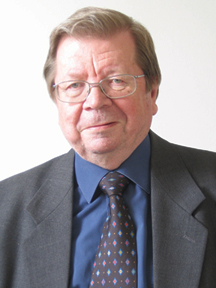
\includegraphics[width=0.25\textwidth]{teuvo}
    \caption{Teuvo Kohonen}
    \label{fig:turing}
\end{wrapfigure}


Además de esto, han surgido otros modelos como las redes neuronales
convolucionales \cite{hubel1968receptive, fukushima1980neocognitron,
  behnke2003hierarchical, lecun1998gradient, graupe1988applications}
la cuál un tipo de red neuronal artificial donde las neuronas
corresponden a campos receptivos de una manera muy similar a las
neuronas en la corteza visual primaria de un cerebro biológico.\\

\textbf{Agregar información sobre las redes neuronales de Google}\\

Con esto se pretende brindar un pequeño contexto histórico e
informativo sobre las redes neuronales. En lo que resta del capítulo
hablaremos brevemente acerca del lenguaje de programación Clojure.

\section{Clojure}

\gls{clojure} es un lenguaje dinámico, de proposito general, que combina el
enfoque y el desarrollo interactivo de un lenguaje de
\textsl{scripting} con una eficiente y robusta infraestructura para
programación multihilo.\\

Además, \gls{clojure} es un lenguaje dialecto de Lisp y comparte con
Lisp la filosofia del código como datos y un sistema poderoso de
macros. Es predominantemente un lenguaje funcional con características
tales como un conjunto rico estructuras de datos inmutables y
persistentes. Cuando es necesario la mutabilidad, Clojure ofrece un
sistema transaccional de memoria y un sistema de agentes reactivos que
garantiza diseños multihilo limpios y correctos.\\

La interfaz principal de desarrollo de Clojure es a través de REPL
(Read-Eval-Print-Loop), la cuál es una simple consola que permite
escribir comandos y examinar sus resultados. Ejemplos sencillos de
código son:

\begin{minted}{clojure}
(def x 6)
-> #'user/x
(def y 36)
-> #'user/y
(+ x y)
-> 42
\end{minted}

Clojure tiene los siguientes tipos de datos: enteros de precisión
arbitraria, cadenas, ratios, caracteres, símbolos, keywords.

\begin{minted}{clojure}
(* 12345678 12345678)
-> 152415765279684
"string"
-> "string"
22/7
-> 22/7
3.14159
-> 3.14159
\a
-> \a
'symbol
-> symbol
:keyword
-> :keyword
;a comment
\end{minted}

\subsection{Programación funcional}

Clojure es un lenguaje de programación funcional. Va a proveer
herramientas para evitar estado mutable, provee funciones de primera
clase y enfatiza en la iteración recursiva en lugar de ciclos con
efectos laterales. Sin embargo, Clojure no es puro, ya que no te forza
a que tu programa sea referencialmente transparente y no se esfuerza
en tener programas que sean ``demostrables''.\\

La filosofía detrás de Clojure es que la mayor parte de los programas
deberían de ser funcionales y los programas que son funcionales son
más robustos.\\

Varias de estas características serán detalladas en el capítulo
\ref{cha:clojure}, donde se explicará a detalle todo lo anterior y con
mayor rigor que el aquí expuesto.